\chapter{ Констукторский раздел}
\label{cha:design}
    В данном разделе будут рассмотрены схемы алгоритмов, требования к функциональности ПО, и определены способы тестирования.
    
    \section{Требования к функциональности ПО}
        В данной работе требуется обеспечить следующую функциональность.
        \begin{enumerate}
            \item Пользовательский режим:
            \begin{enumerate}
                \item возможность подать на вход матрицу точек;
                \item вывод результата работы алгоритмов.
            \end{enumerate}
	\item Тестовый режим: 
            \begin{enumerate}
            	\item возможность замера процессорного времени реализации алгоритма с параллельными вычислениями с варьируемым количеством потоков.
            \end{enumerate}
        \end{enumerate}
	
	\section{Схемы алгоритмов}
        Ниже будут представлены схемы алгоритмов: \begin{enumerate}
            \item последовательный k-means (рисунок \ref{schema:Fuzzy});
            \item параллельный k-means (рисунок \ref{schema:FuzzyPar}).
        \end{enumerate}
      
       	    \begin{figure}[h!]
       		\centering
       		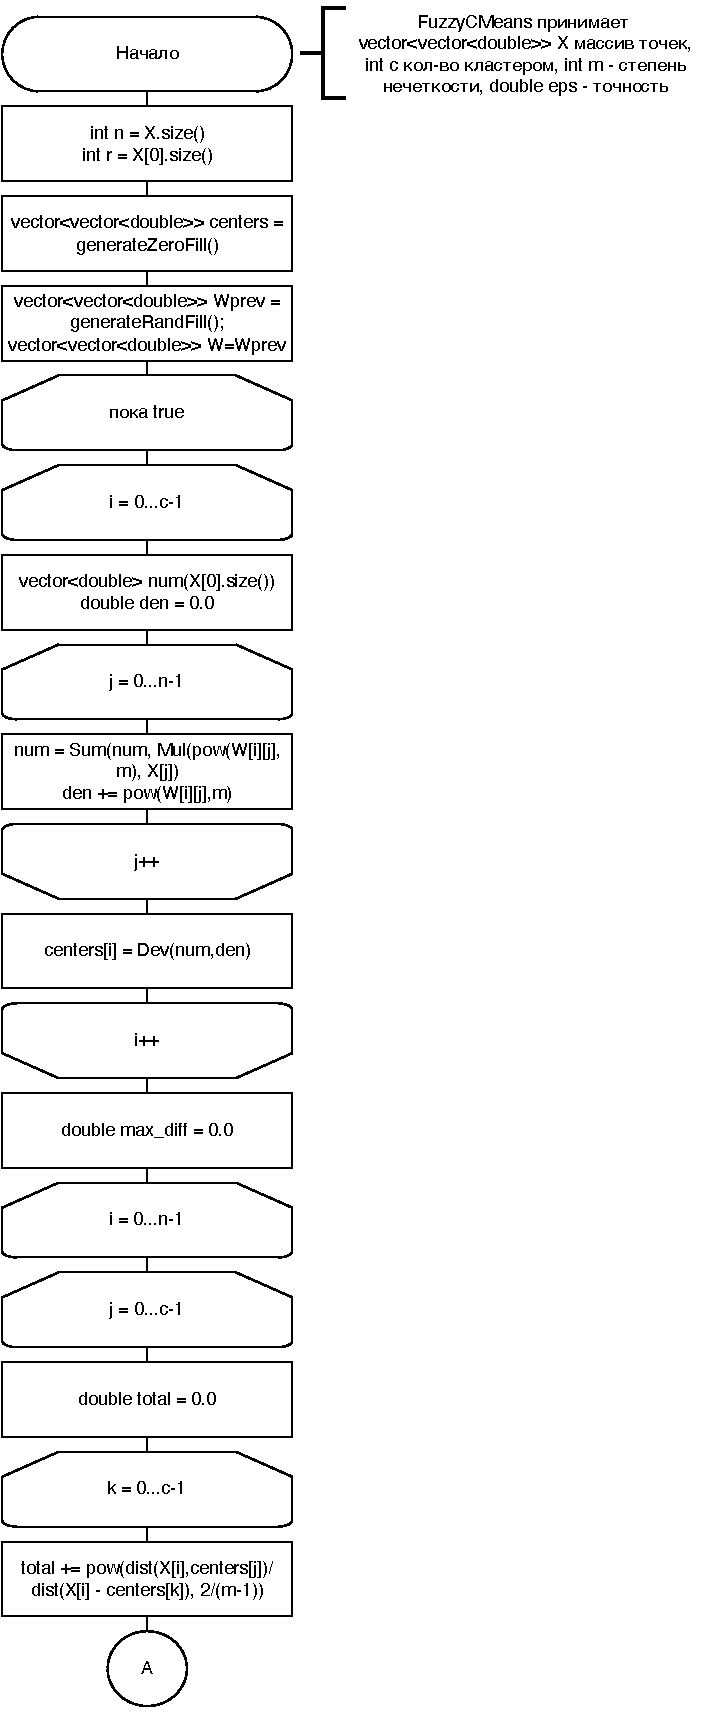
\includegraphics[scale=0.8]{Fuzzy.pdf}
       		\caption{Последовательный нечеткий алгоритм с-средних Часть 1}
       		\label{schema:Fuzzy}
       	\end{figure}\clearpage
        \begin{figure}[h!]
            \centering
            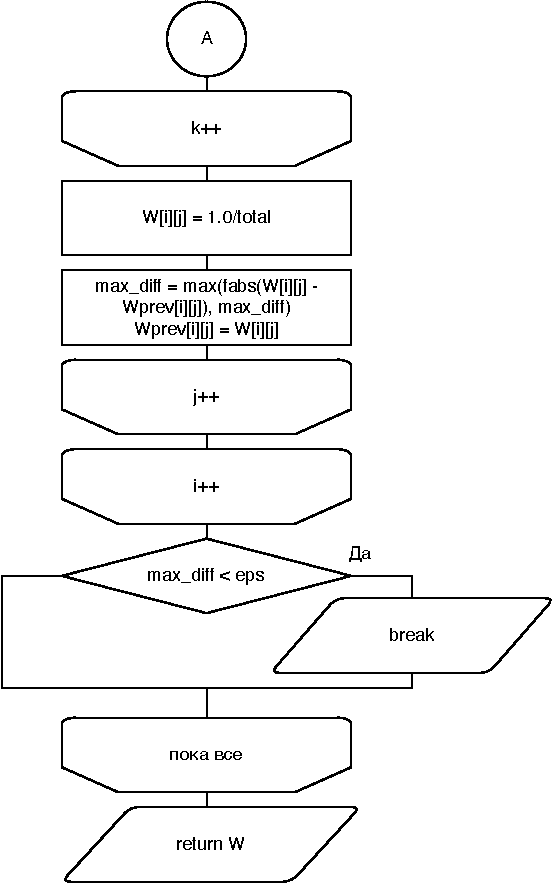
\includegraphics[scale=0.8]{Fuzzy_1.pdf}
            \caption{Последовательный нечеткий алгоритм с-средних Часть 2}
            \label{schema:Fuzzy_1}
        \end{figure}\clearpage
       	
       	\begin{figure}[h!]
            \centering
            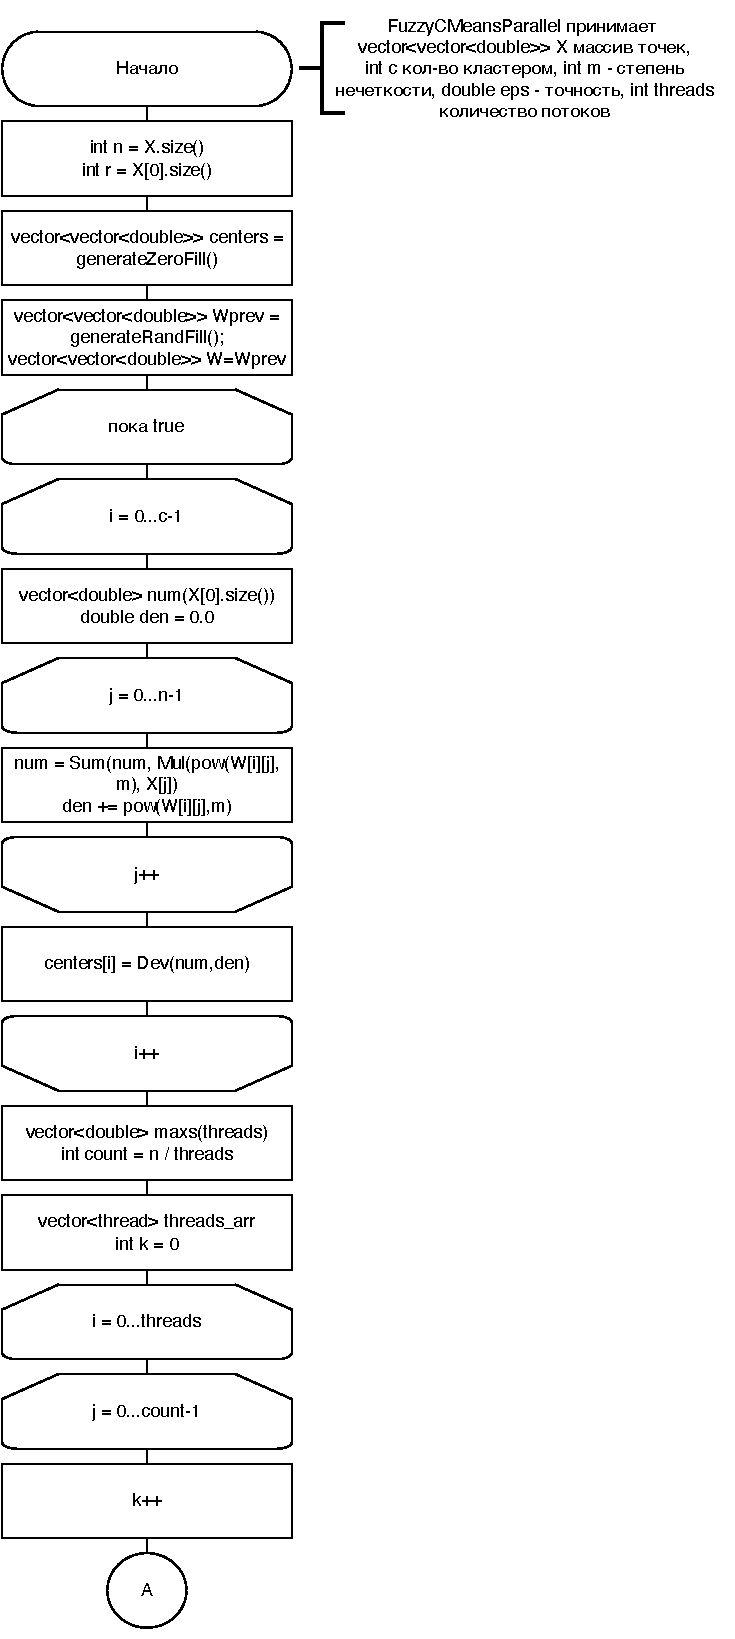
\includegraphics[scale=0.8]{FuzzyPar.pdf}
            \caption{Параллельный нечеткий алгоритм с-средних Часть 1}
            \label{schema:FuzzyPar}
        \end{figure}\clearpage
        \begin{figure}[h!]
            \centering
            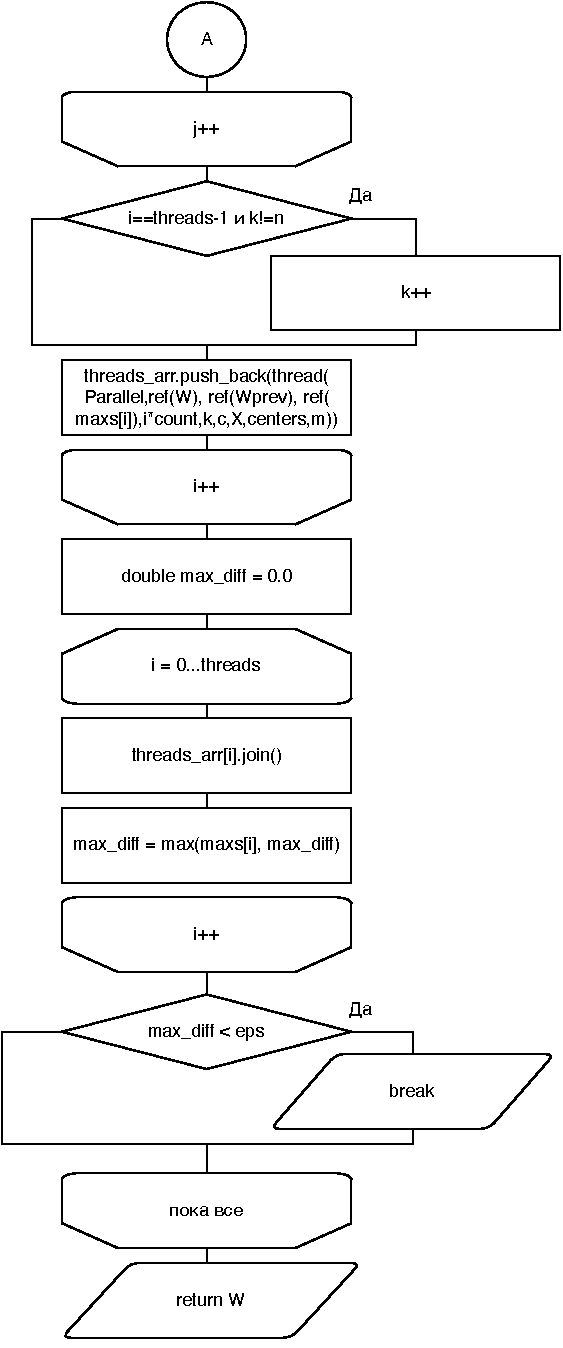
\includegraphics[scale=0.8]{FuzzyPar_1.pdf}
            \caption{Параллельный нечеткий алгоритм с-средних Часть 2}
            \label{schema:FuzzyPar_1}
        \end{figure}\clearpage
    \section{Тесты}
    Тестирование ПО будет проводиться методом чёрного ящика. Необходимо проверить работу системы 
    на массивах различной длины.
  	

	\section*{Вывод}
    \par На основе теоретических данных, полученных из аналитического раздела, была построена схема нечёткого алгоритма k-means, а так же после разделения алгоритма на этапы была предложена схема параллельного выполнения данных этапов.
\newpage